\documentclass[11pt,a4paper]{article}
\usepackage[T1]{fontenc}
\usepackage[utf8]{inputenc}
\usepackage[french]{babel}
\usepackage[left=2cm,right=2cm,top=2cm,bottom=2cm]{geometry}
\usepackage{amsmath}
\usepackage{amsfonts}
\usepackage{amssymb}
\usepackage{amsthm}
\usepackage{stmaryrd}
\usepackage{graphicx}
\usepackage{booktabs}
\usepackage{bbold}
\usepackage{minted}
\usepackage{colortbl}
\usepackage{multirow}
\usepackage{diagbox}
\usepackage{forest}
\usepackage{enumitem}
\usepackage{here}
\usepackage{hyperref}
\usepackage{subcaption}
\newtheorem{lemme}{\textit{Lemme}}

\author{\DIAS Pierre}
\date{ }
\title{\begin{huge} \textbf{DM1}\end{huge}}
\usepackage[tikz]{bclogo}
\usepackage{xcolor}
\begin{document}
\begin{titlepage}

\newcommand{\HRule}{\rule{\linewidth}{0.5mm}}
\center 


\begin{figure}
    \centering
    
\includegraphics[width=0.5\linewidth]{images_plot/ssd_logo_couleur_noir-300x103.png}
\end{figure}



\textsc{\Large Master 2 Statistiques et Sciences des Données }\\[1cm] % Major heading such as course name
\HRule \\[0.4cm]
{ \huge \bfseries Compte Rendu TP \\  SVM}\\[0.4cm]
\HRule \\[1.5cm]
\begin{center}
\begin{Large}
DIAS Pierre
\end{Large}
\end{center}
    

\begin{center}

\vfill{\includegraphics[width=0.1\linewidth]{images_plot/Logo_université_montpellier.png}\vspace{0.5cm}\\
\begin{Large} Année 2024 - 2025 \\
\end{Large}}



\end{center}

\end{titlepage}
\pagebreak

\tableofcontents
\pagebreak


\section{Introduction}
 Dans ce TP, nous allons étudier la méthode SVM (Support Vector Machine) notemment utilisée
 pour la classification, la régression ou encore la détection d’anomalies. Nous allons utiliser la
 librairie \colorbox{gray!15}{\textit{scikit-learn}} pour implémenter cette méthode.

\section{Mise en oeuvre}
 
Nous cherchons à classifier les instances des classes 1 et 2 en utilisant uniquement les deux premières variables du dataset \textit{IRIS} (longueur et largeur des sépales). Une évaluation de la performance du modèle est effectuée en utilisant une validation croisée, en laissant la moitié des données pour l'entraînement et l'autre moitié pour le test.

\subsection{Question 1: Classification du dataset \texttt{iris}}

Pour classifier un dataset, nous mélangeons les données, puis les séparons en deux ensembles distincts : un ensemble d'entraînement et un ensemble de test. Ensuite, nous pouvons obtenir les scores relatifs à ces deux ensembles.

\begin{minted}[bgcolor=pink!10]{python}
X, y = shuffle(X, y, random_state=i)
X_train, X_test, y_train, y_test = train_test_split(X, y,test_size=0.5, 
random_state=i)
# Initialisation du modèle SVM avec noyau linéaire
clf_linear = SVC(kernel='linear', C=1.0)
# Entraînement du modèle
clf_linear.fit(X_train, y_train)
\end{minted}

Après avoir itéré l'expérience 1000 fois, nous obtenons les résultats de score suivants:
\begin{itemize}
    \item Moyenne des scores d'entraînement pour le noyau linéaire: 0.7216
    \item Moyenne des scores de test pour le noyau linéaire: 0.6859
\end{itemize}

Cela implique que le modèle a bien appris à classifier les instances dans les données d'entraînement avec une précision de 72\%. Cependant il est capable de généraliser cela avec une précision de 68,6\% ce qui implique une légère sur-adaptation aux données d'entraînement. Cela pourrait être amélioré en ajustant le paramètre \colorbox{gray!15}{\textit{C}}.

\subsection{Question 2: Comparaison des noyaux}

Il est possible de comparer des différents noyaux pour la classification. Ici nous avons comparé un noyau linéraires avec un noyau polynomial de degrés 1,2 et 3. 

\begin{minted}[bgcolor=pink!10]{python}
Cs = list(map(float, np.logspace(-3, 3, 5)))
gammas = list(map(float, 10. ** np.arange(1, 2)))
degrees = list(map(int, np.r_[1, 2, 3]))
# Définition du grid de paramètres
parameters = {'kernel': ['poly'], 'C': Cs, 'gamma': gammas, 'degree': degrees}
# Utilisation de GridSearchCV
clf_poly = GridSearchCV(SVC(), param_grid=parameters, n_jobs=-1)
clf_poly.fit(X_train, y_train)
\end{minted}



On obtient ainsi les meilleurs paramètres:

\textit{'C': 0.0316, 'degree': 1, 'gamma': 10.0, 'kernel': 'poly'}

\pagebreak
\begin{figure}[H]
    \centering
    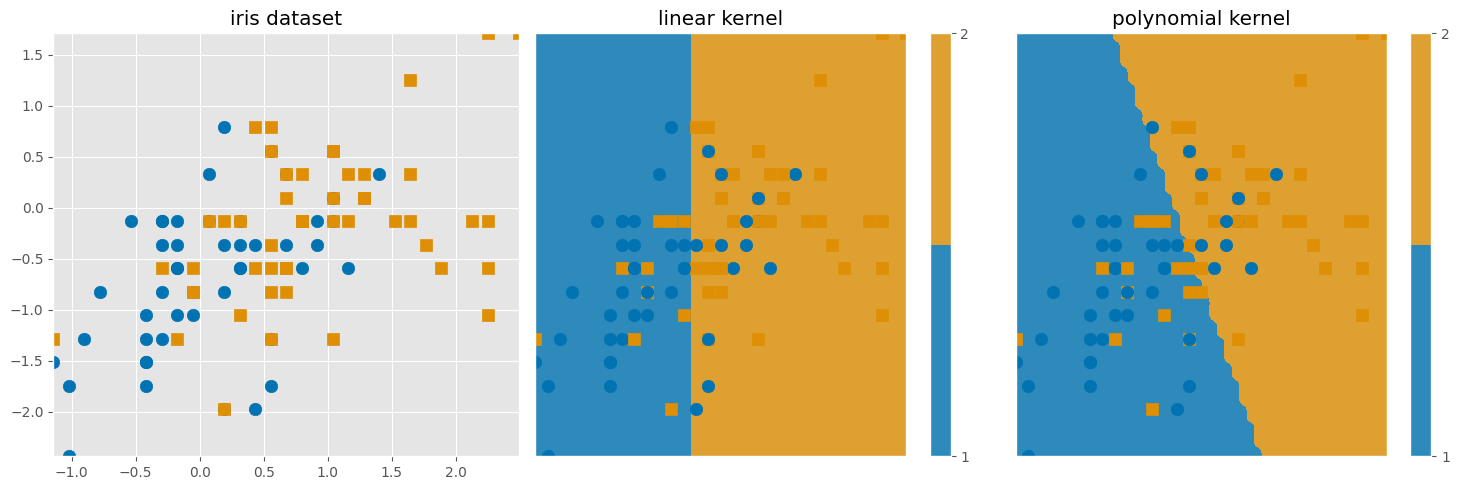
\includegraphics[width=1\linewidth]{images_plot/compar_lin_poly.png}
    \caption{Comparaison entre un noyau linéaire et un noyau polynomial}
    \label{fig1}
\end{figure}

Il est possible de faire apparaître les frontières sur le jeu de données. On comprend que le meilleur choix de noyau était bien un noyau polynomial mais d'ordre 1! Cela dépend beaucoup de l'aléatoire lorsque nous mélangeons nos données.

\section{SVM GUI - Question 3}

L'application \texttt{svm\_gui.py} de Scikit-learn permet d'évaluer en temps réel l'impact du choix du noyau (linéaire, polynomial, RBF) et du paramètre de régularisation \(C\) sur les performances d'un modèle SVM. En générant un jeu de données très déséquilibré (90\% vs 10\%), il est possible de visualiser comment les paramètres influent sur le modèle.



\begin{figure}[H]
    \centering
    \begin{minipage}{0.24\textwidth}
        \centering
        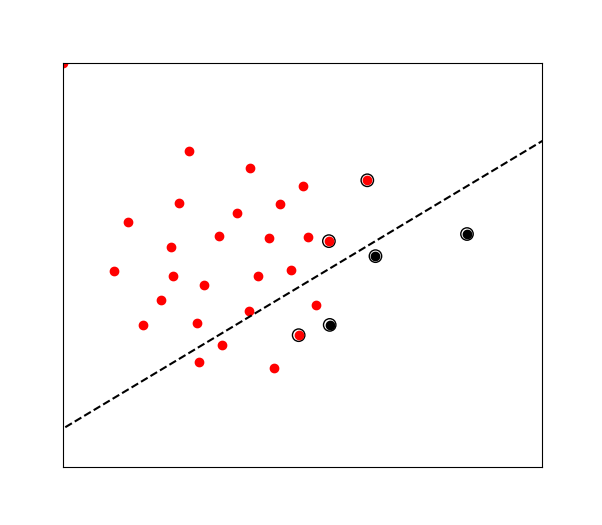
\includegraphics[width=\textwidth]{images_plot/C001.png}
        \caption*{C=0,01}
    \end{minipage}
    \hfill
    \begin{minipage}{0.24\textwidth}
        \centering
        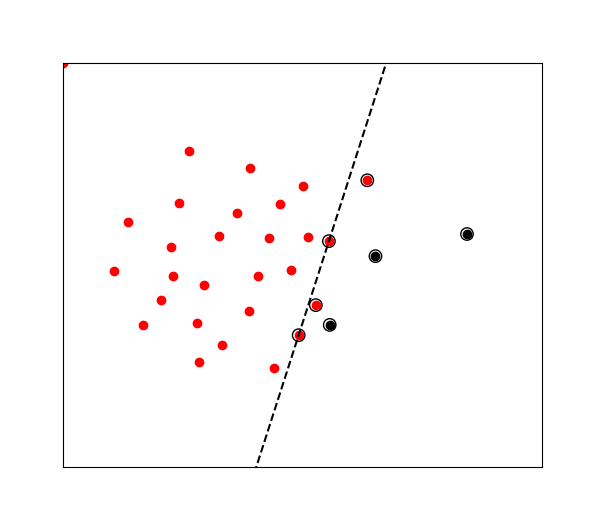
\includegraphics[width=\textwidth]{images_plot/C1.png}
        \caption*{C=1}
    \end{minipage}
    \hfill
    \begin{minipage}{0.24\textwidth}
        \centering
        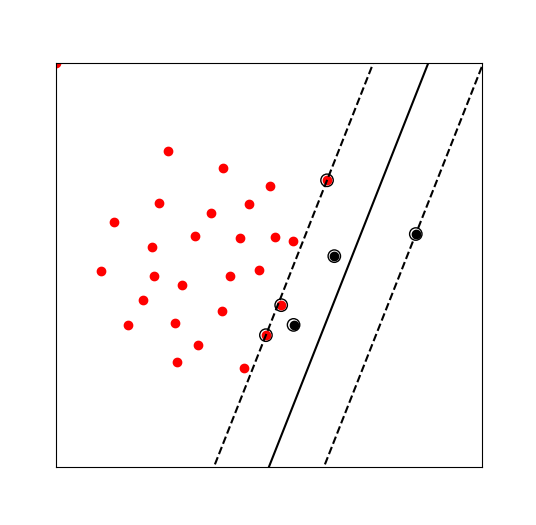
\includegraphics[width=\textwidth]{images_plot/C100.png}
        \caption*{C=100}
    \end{minipage}
    \hfill
    \begin{minipage}{0.24\textwidth}
        \centering
        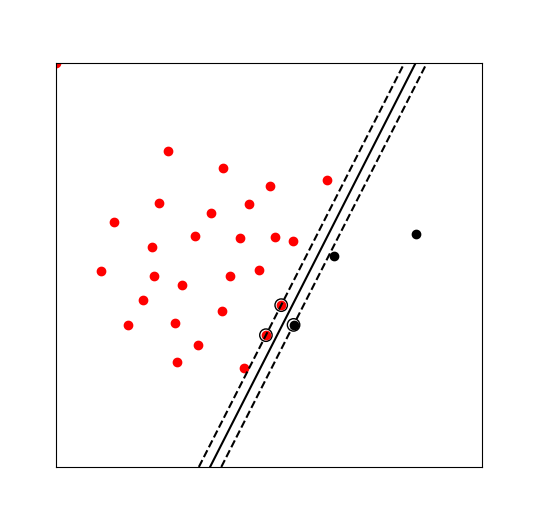
\includegraphics[width=\textwidth]{images_plot/C10000.png}
        \caption*{C=10000}
    \end{minipage}
    \caption{Utilisation de SVM\_gui pour différentes valeurs de C}
\end{figure}

En jouant avec le paramètre C, nous voyons bien que plus celui ci est grand, moins le modèle accepte d'individus dans la marge et inversement. 

\pagebreak
\section{Classification des visages}

Pour cette partie, nous nous intéresserons à la reconnaissance faciale au travers des SVM que l'on qualifiera de classification des visages. 
Pour cela nous utiliserons la base de données \texttt{LFW} (\url{http://vis-www.cs.umass.edu/lfw/lfw-funneled.tgz}), en sélectionnant uniquement les images de Tony Blair et Colin Powell pour effectuer ensuite classification binaire.

\begin{figure}[H]
    \centering
    \includegraphics[width=0.5\linewidth]{images_plot/visages.png}
    \caption{Échantillon de la base de donnée}
    \label{fig:enter-label}
\end{figure}


\subsection{Question 4: Influence du paramètre C}

Après avoir divisé nos données en deux échantillons, l'un pour l'entraînement et l'autre pour le test, nous souhaitons démontrer l'influence du paramètre de régularisation.
Nous pouvons observer l'effet du choix de C sur les performances du modèle de la manière suivante:

\begin{figure}[H]
    \centering
    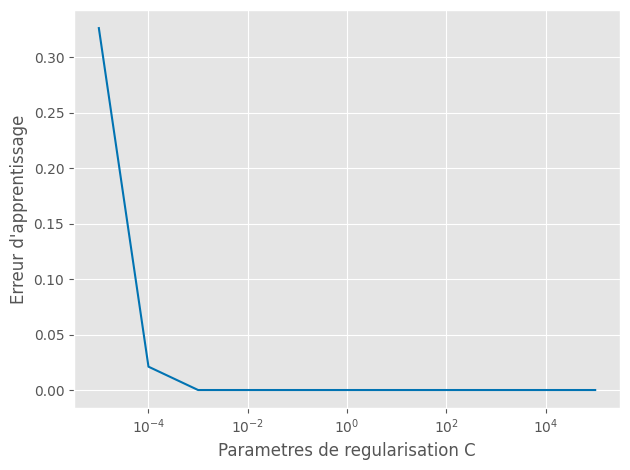
\includegraphics[width=0.5\linewidth]{images_plot/Erreur.png}
    \caption{Erreur d'apprentissage en fonction du choix de C}
    \label{fig:enter-label}
\end{figure}
On obtient donc que le meilleurs C pour ce modèle est de $0.001$ soit $10^{-3}$ qui permet de réduire l'erreur à $0$. Cela implique donc un score de $1$ qui est parfait pour la prédiction des noms selon les images.

\begin{figure}[H]
    \centering
    \begin{minipage}{0.45\textwidth}
        \centering
        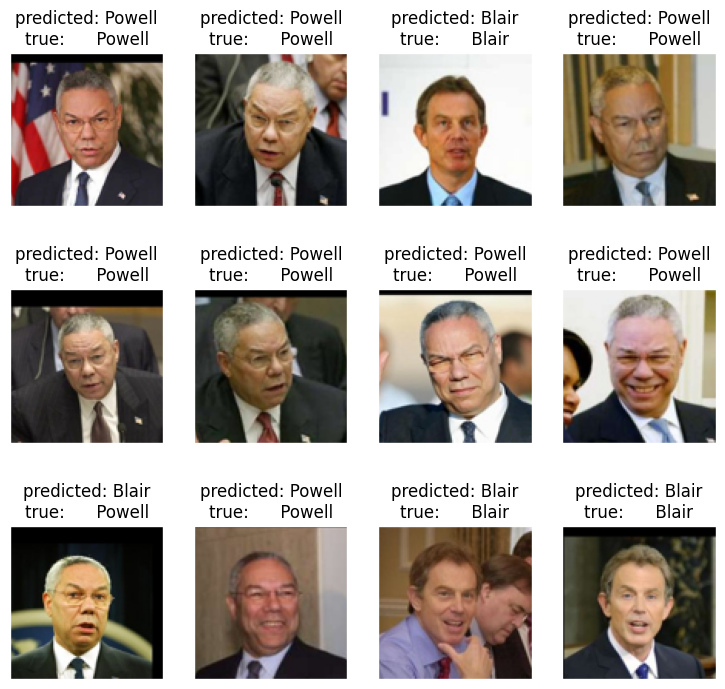
\includegraphics[width=\textwidth]{images_plot/predictnom.png}
        \caption{Échantillon de prédictions}
        \label{fig:image1}
    \end{minipage}
    \hfill
    \begin{minipage}{0.45\textwidth}
        \centering
        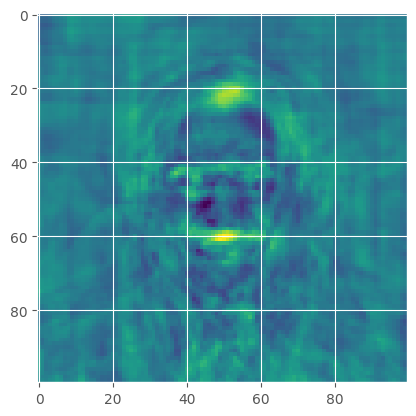
\includegraphics[width=\textwidth]{images_plot/heatmap.png}
        \caption{Zones importantes pour la reconnaissance faciale}
        \label{fig:image2}
    \end{minipage}
    \label{fig:images}
\end{figure}

D'après les résultats obtenus dans le cadre du travail pratique (Figure~\ref{fig:image1}), toutes les prédictions se sont avérées correctes, à l'exception de la neuvième dans cet échantillon.

De plus, nous avons calculé les métriques suivantes :

\begin{table}[H]
    \centering
    \begin{tabular}{|cc|}
        \hline
        \textbf{Métrique}     & \textbf{Valeur} \\ \hline
        Chance level          & 0.62            \\
        Accuracy              & 0.89            \\ \hline
    \end{tabular}
    \caption{Métriques de performance du modèle}
    
    \label{table1}
\end{table}
Le niveau de hasard correspond à l'exactitude qui sera atteinte en prédisant constamment la classe majoritaire.
Ces résultats (Table~\ref{table1}) montrent que le modèle présente une précision (\textit{Accuracy}) supérieure au niveau de chance (\textit{Chance level}) ce qui veut dire que le modèle est plutot fiable. 

Enfin, la Figure~\ref{fig:image2} illustre les zones importantes du visage pour la reconnaissance faciale, mettant en évidence des éléments tels que la forme du visage, les yeux, la bouche et le haut du crâne.

\subsection{Question 5: Modèle avec nuisance}

Nous allons ajouter des variables de nuisances dans notre modèle, ce qui augmentera le nombre total de variables tout en maintenant constant le nombre de points d'apprentissage. L'objectif est de démontrer comment cette augmentation des variables de nuisances peut entraîner une chute significative des performances du modèle.

\begin{minted}[bgcolor=pink!10]{python}
noise = sigma * np.random.randn(n_samples, 300, )
X_noisy = np.concatenate((X, noise), axis=1)
X_noisy = X_noisy[np.random.permutation(X.shape[0])]
\end{minted}

Nous avons évalué notre modèle en deux scénarios : sans variable de nuisance et avec variable de nuisance. Les scores de généralisation pour chaque cas sont les suivants :

\begin{table}[H]
    \centering
    \begin{tabular}{|ccc|}
        \hline
\textbf{Condition}& \textbf{Score d'Entraînement} & \textbf{Score de Test} \\ \hline
        Sans variable de nuisance& 1.0 & 0.8947  \\
        Avec variable de nuisance  & 1.0                           & 0.5368\\                 \hline
    \end{tabular}
    \caption{Scores de Généralisation pour le modèle avec et sans Variable de Nuisance}
    \label{table2}
\end{table}

Dans le premier cas (Table~\ref{table2}), nous observons que le modèle atteint un score de généralisation de 1.0 sur l'échantillon d'entraînement et 0.8947 sur l'échantillon de test. En revanche, lorsque nous introduisons des variables de nuisance, bien que le score d'entraînement reste à 1.0, le score de test chute à 0.5368. Cela suggère que les variables de nuisance affectent significativement la capacité du modèle à généraliser sur de nouvelles données.



\subsection{Question 6: Amélioration de la prédiction par réduction de dimension}

Nous pouvons alors réduire les dimensions pour la prédiction afin de l'améliorer:

\begin{minted}[bgcolor=pink!10]{python}
n_components = 50  # jouer avec ce parametre
pca = PCA(n_components=n_components,svd_solver="randomized").fit(X_noisy)
# On applique PCA sur les données avec bruit
X_noisy_pca = pca.fit_transform(X_noisy)
\end{minted}


\begin{figure}[H]
    \centering
    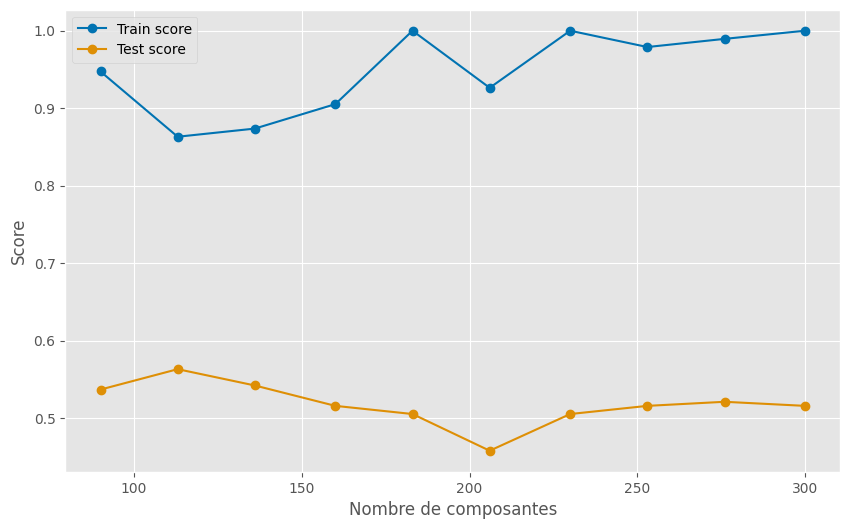
\includegraphics[width=0.7\linewidth]{images_plot/graphPCA.png}
    \caption{Score en fonction du nombre de composantes de l'ACP}
    \label{fig:q6}
\end{figure}

Il aurait été souhaitable de tester un nombre de composantes plus bas, mais les capacités de mon ordinateur ne le permettaient pas.
Sur cette figure~\ref{fig:q6}, nous ne pouvons pas vraiment dégager de conclusion si ce n'est que plus on a de composantes plus le score d'entraînement est proche de 1 mais cela n'est pas vraiment clair.

\end{document}
